\begin{figure}[t]
  \centering
  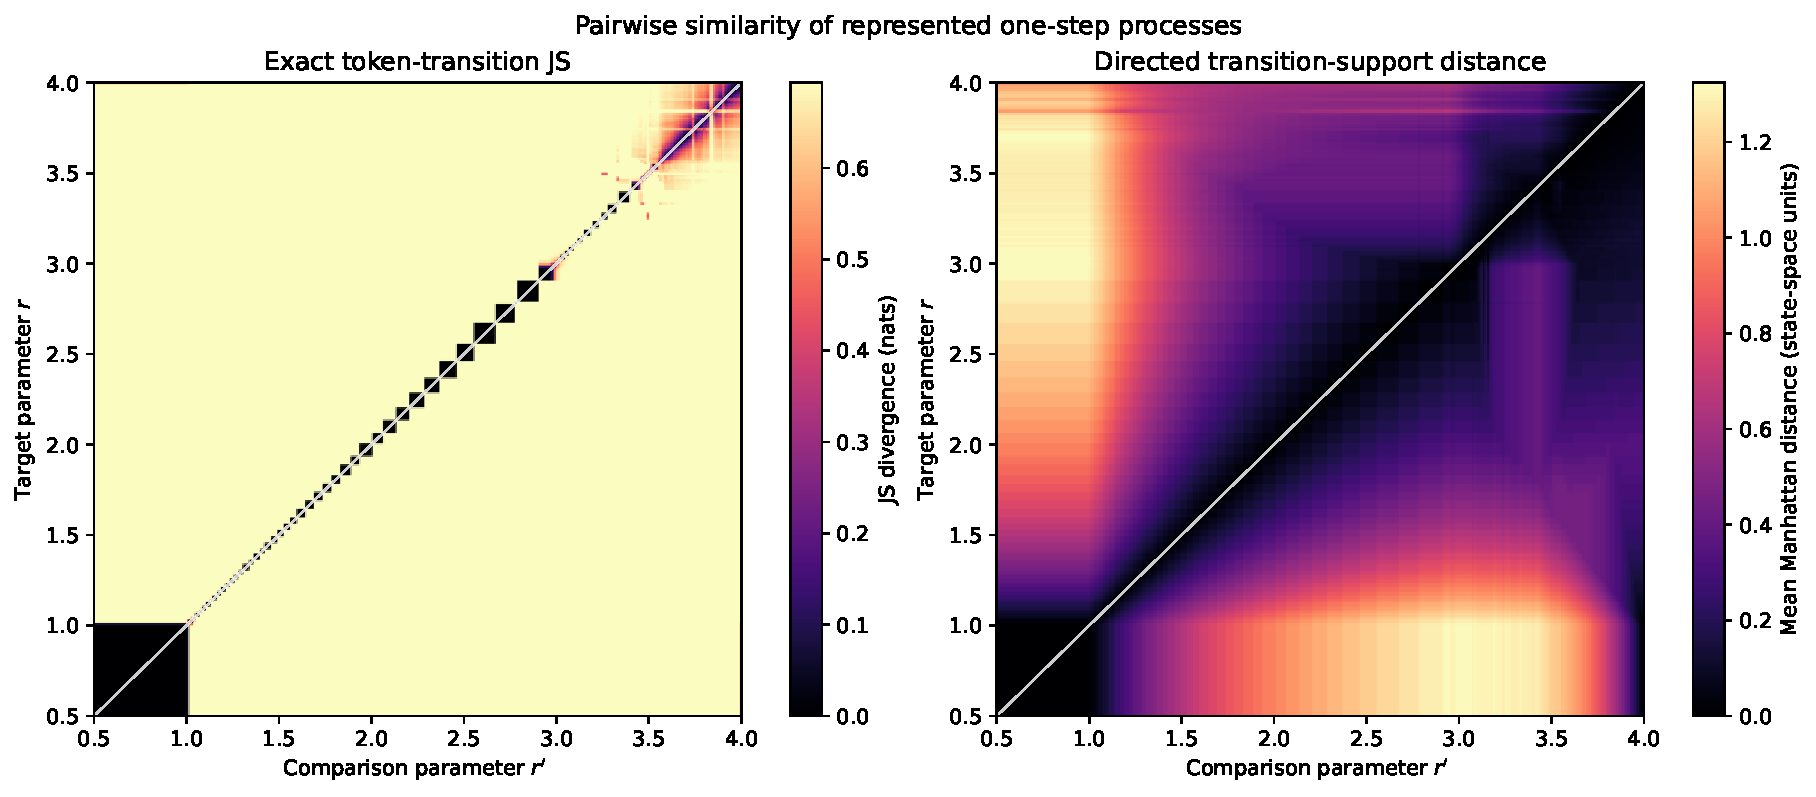
\includegraphics[width=\linewidth]{window_transition_js_matrix.pdf}
  \caption{\textbf{Pairwise similarity of represented one-step processes across
  the logistic family.}
  For each parameter $r$, we estimate the joint token-transition distribution
  $J_r(i,j)=\Pr(t_n=i,t_{n+1}=j\mid r)$ using the same $64$-bin tokenization
  and finite-trajectory protocol used in the restricted-support experiments.
  Rows denote the target parameter $r$ and columns the comparison parameter
  $r'$. \emph{Left:} Jensen--Shannon divergence between $J_r$ and $J_{r'}$;
  this quantity is symmetric. \emph{Right:} directed transition-support
  distance from $r$ to $r'$, defined as
  $D_{\mathrm{supp}}(r,r')=\sum_{i,j}J_r(i,j)
  \min_{(k,\ell)\in\operatorname{supp}(J_{r'})}
  (|i-k|+|j-\ell|)/64$.
  It measures how far the target transition mass lies from transitions
  represented by the comparison system and is therefore generally asymmetric.
  Darker values indicate more similar represented processes; both quantities
  vanish on the diagonal. Each $J_r$ is estimated from $512$ trajectories.}
  \label{fig:window-transition-js-matrix}
\end{figure}
